%\pagebreak

\subsection{Evidencia de realizaci\'on}
Como evidencia se presentan los videos de cada configuraci\'on del motor DC, as\'i como fotograf\'ias que 
detallan la construcci\'on del motor de excitaci\'on separada.

\subsubsection{Videos}
\begin{itemize}
 \item Excitaci\'on separada: https://goo.gl/Xshuqv
 \item Autoexcitaci\'on: https://goo.gl/7YjOCh
 \item Serie: https://goo.gl/MNwQjI
 \item Compuesto: https://goo.gl/GuZF9r
\end{itemize}

\subsubsection{Im\'agenes}
Las fotograf\'ias incluyen la primer iteraci\'on del rotor para el motor DC de excitaci\'on separada,
y las dos versiones ensambladas del motor.

\begin{figure}[!htbp]
\caption{Construcci\'on de motor DC en excitaci\'on separada}
\centering
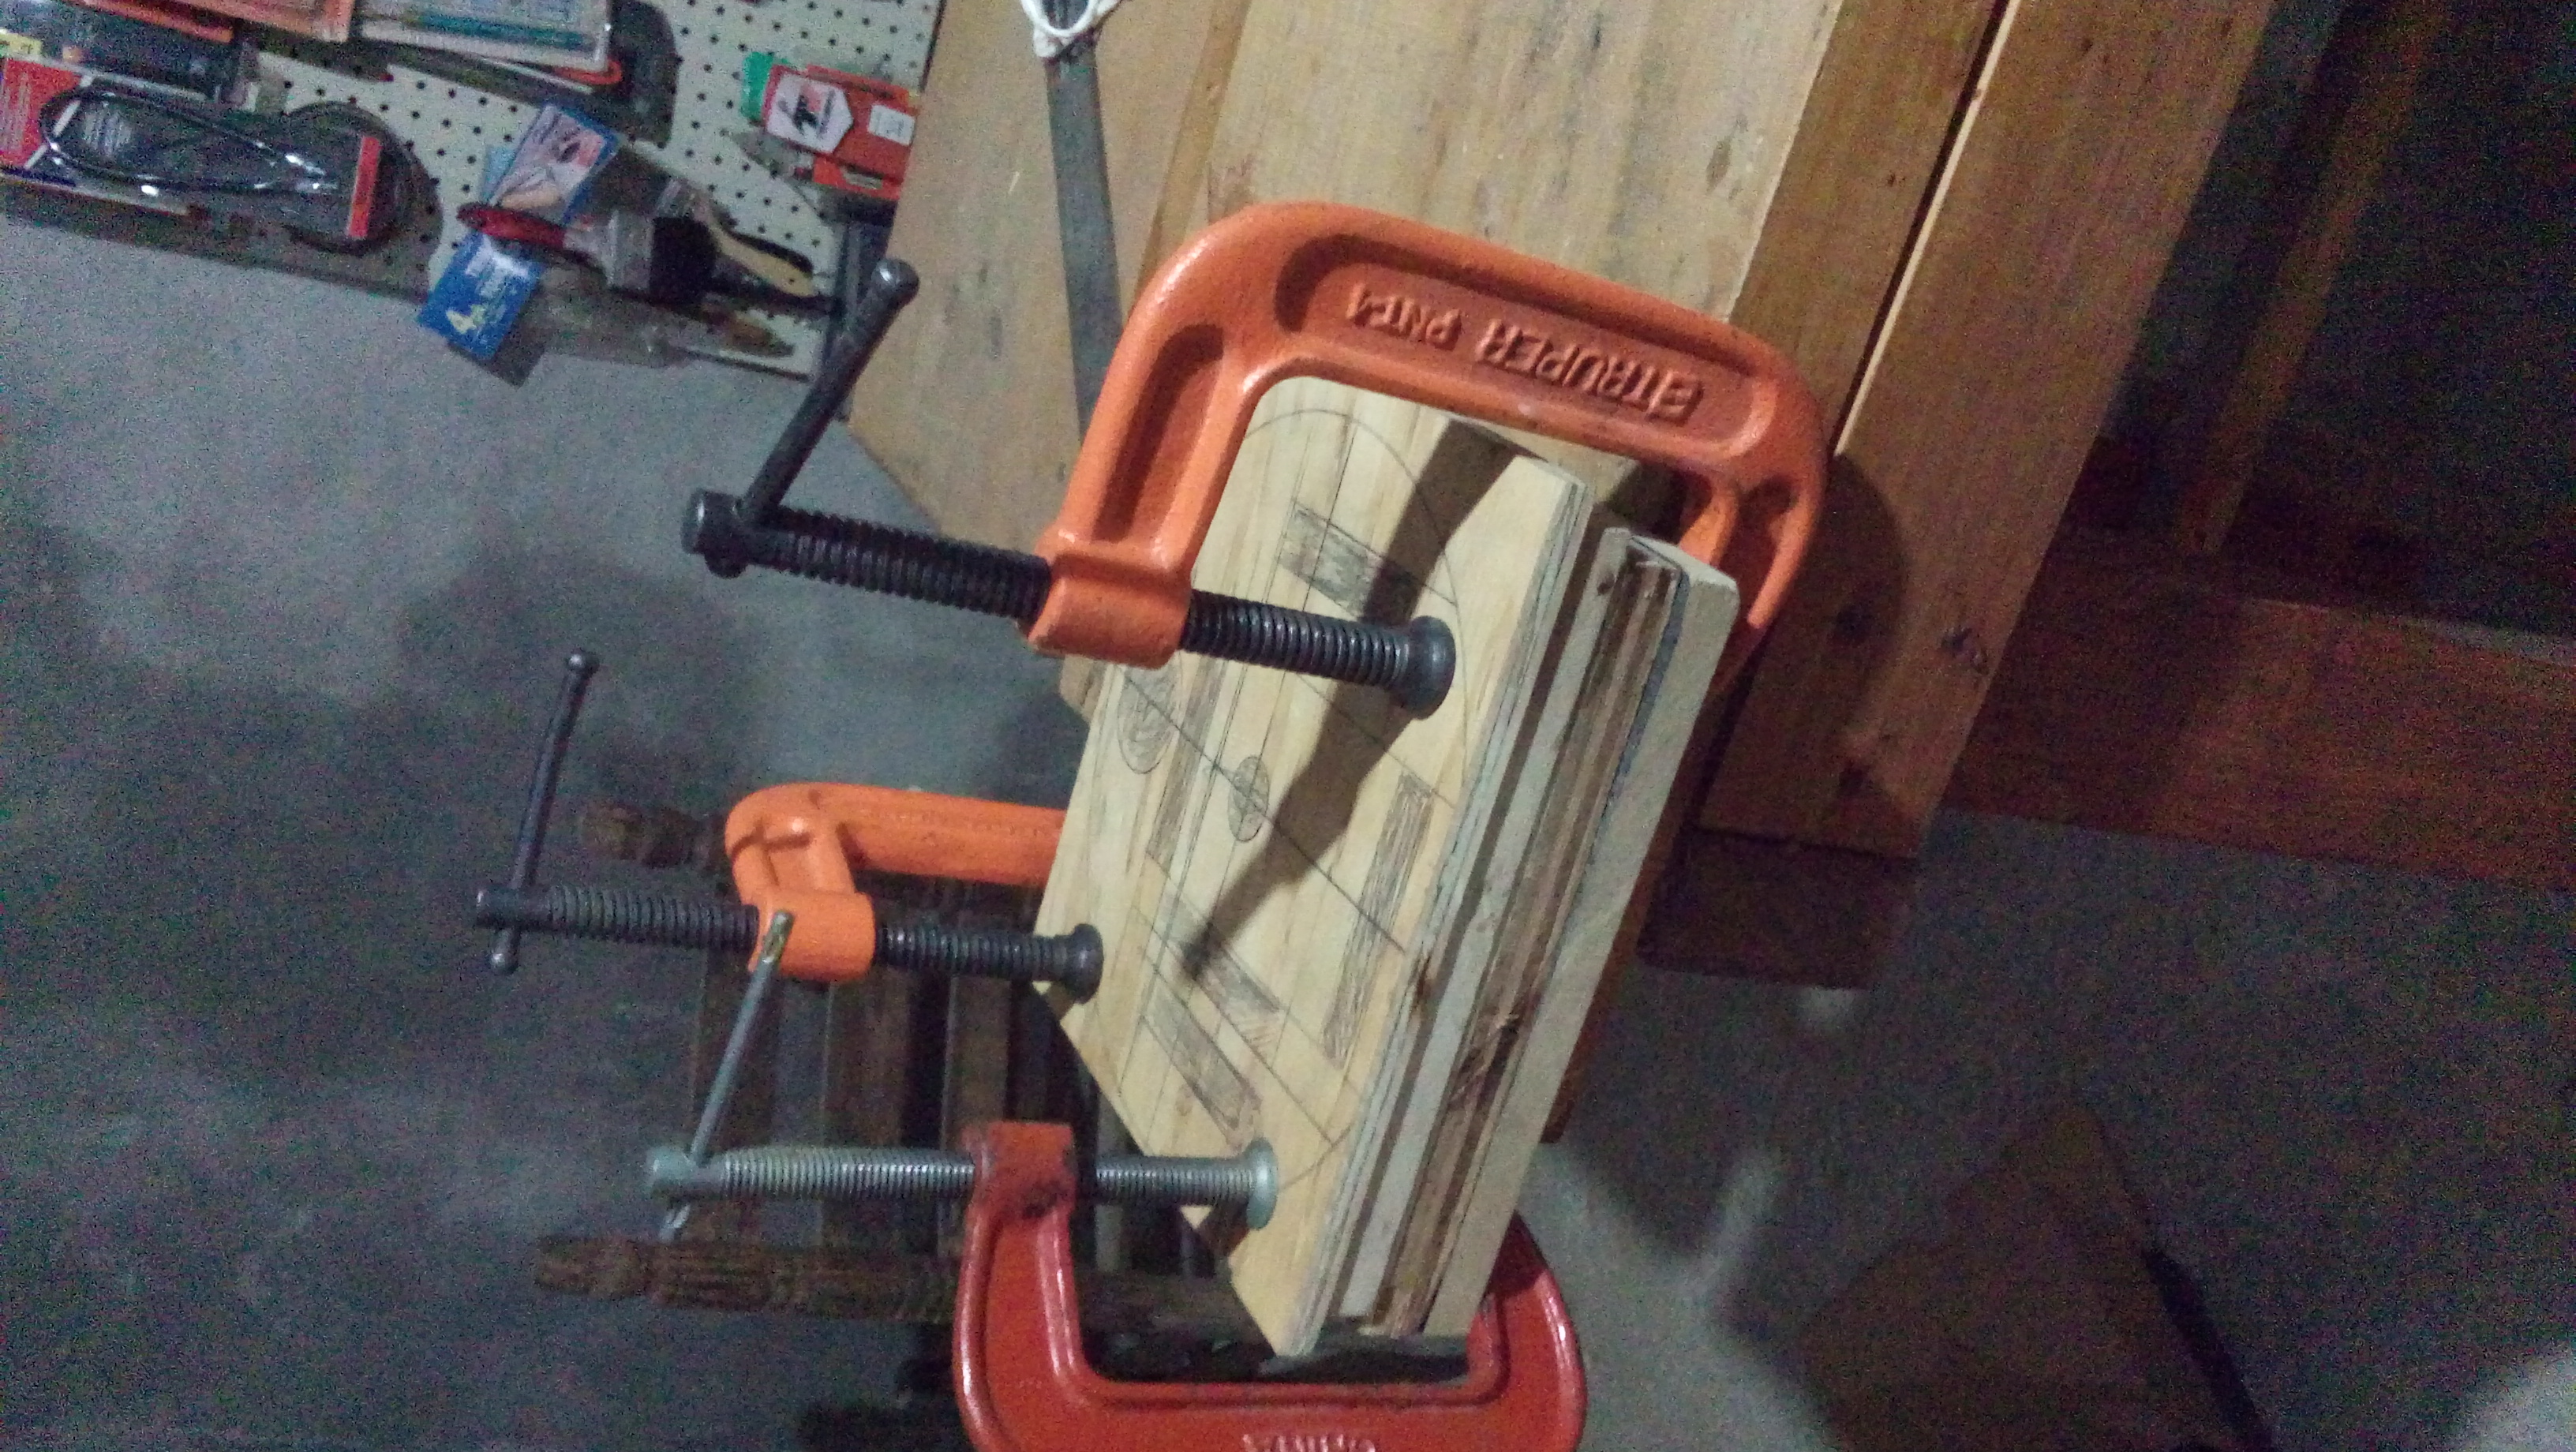
\includegraphics [scale=0.10]
{./img/20160228_190845.jpg}
\end{figure}

\begin{figure}[!htbp]
\caption{Primer rotor}
\centering
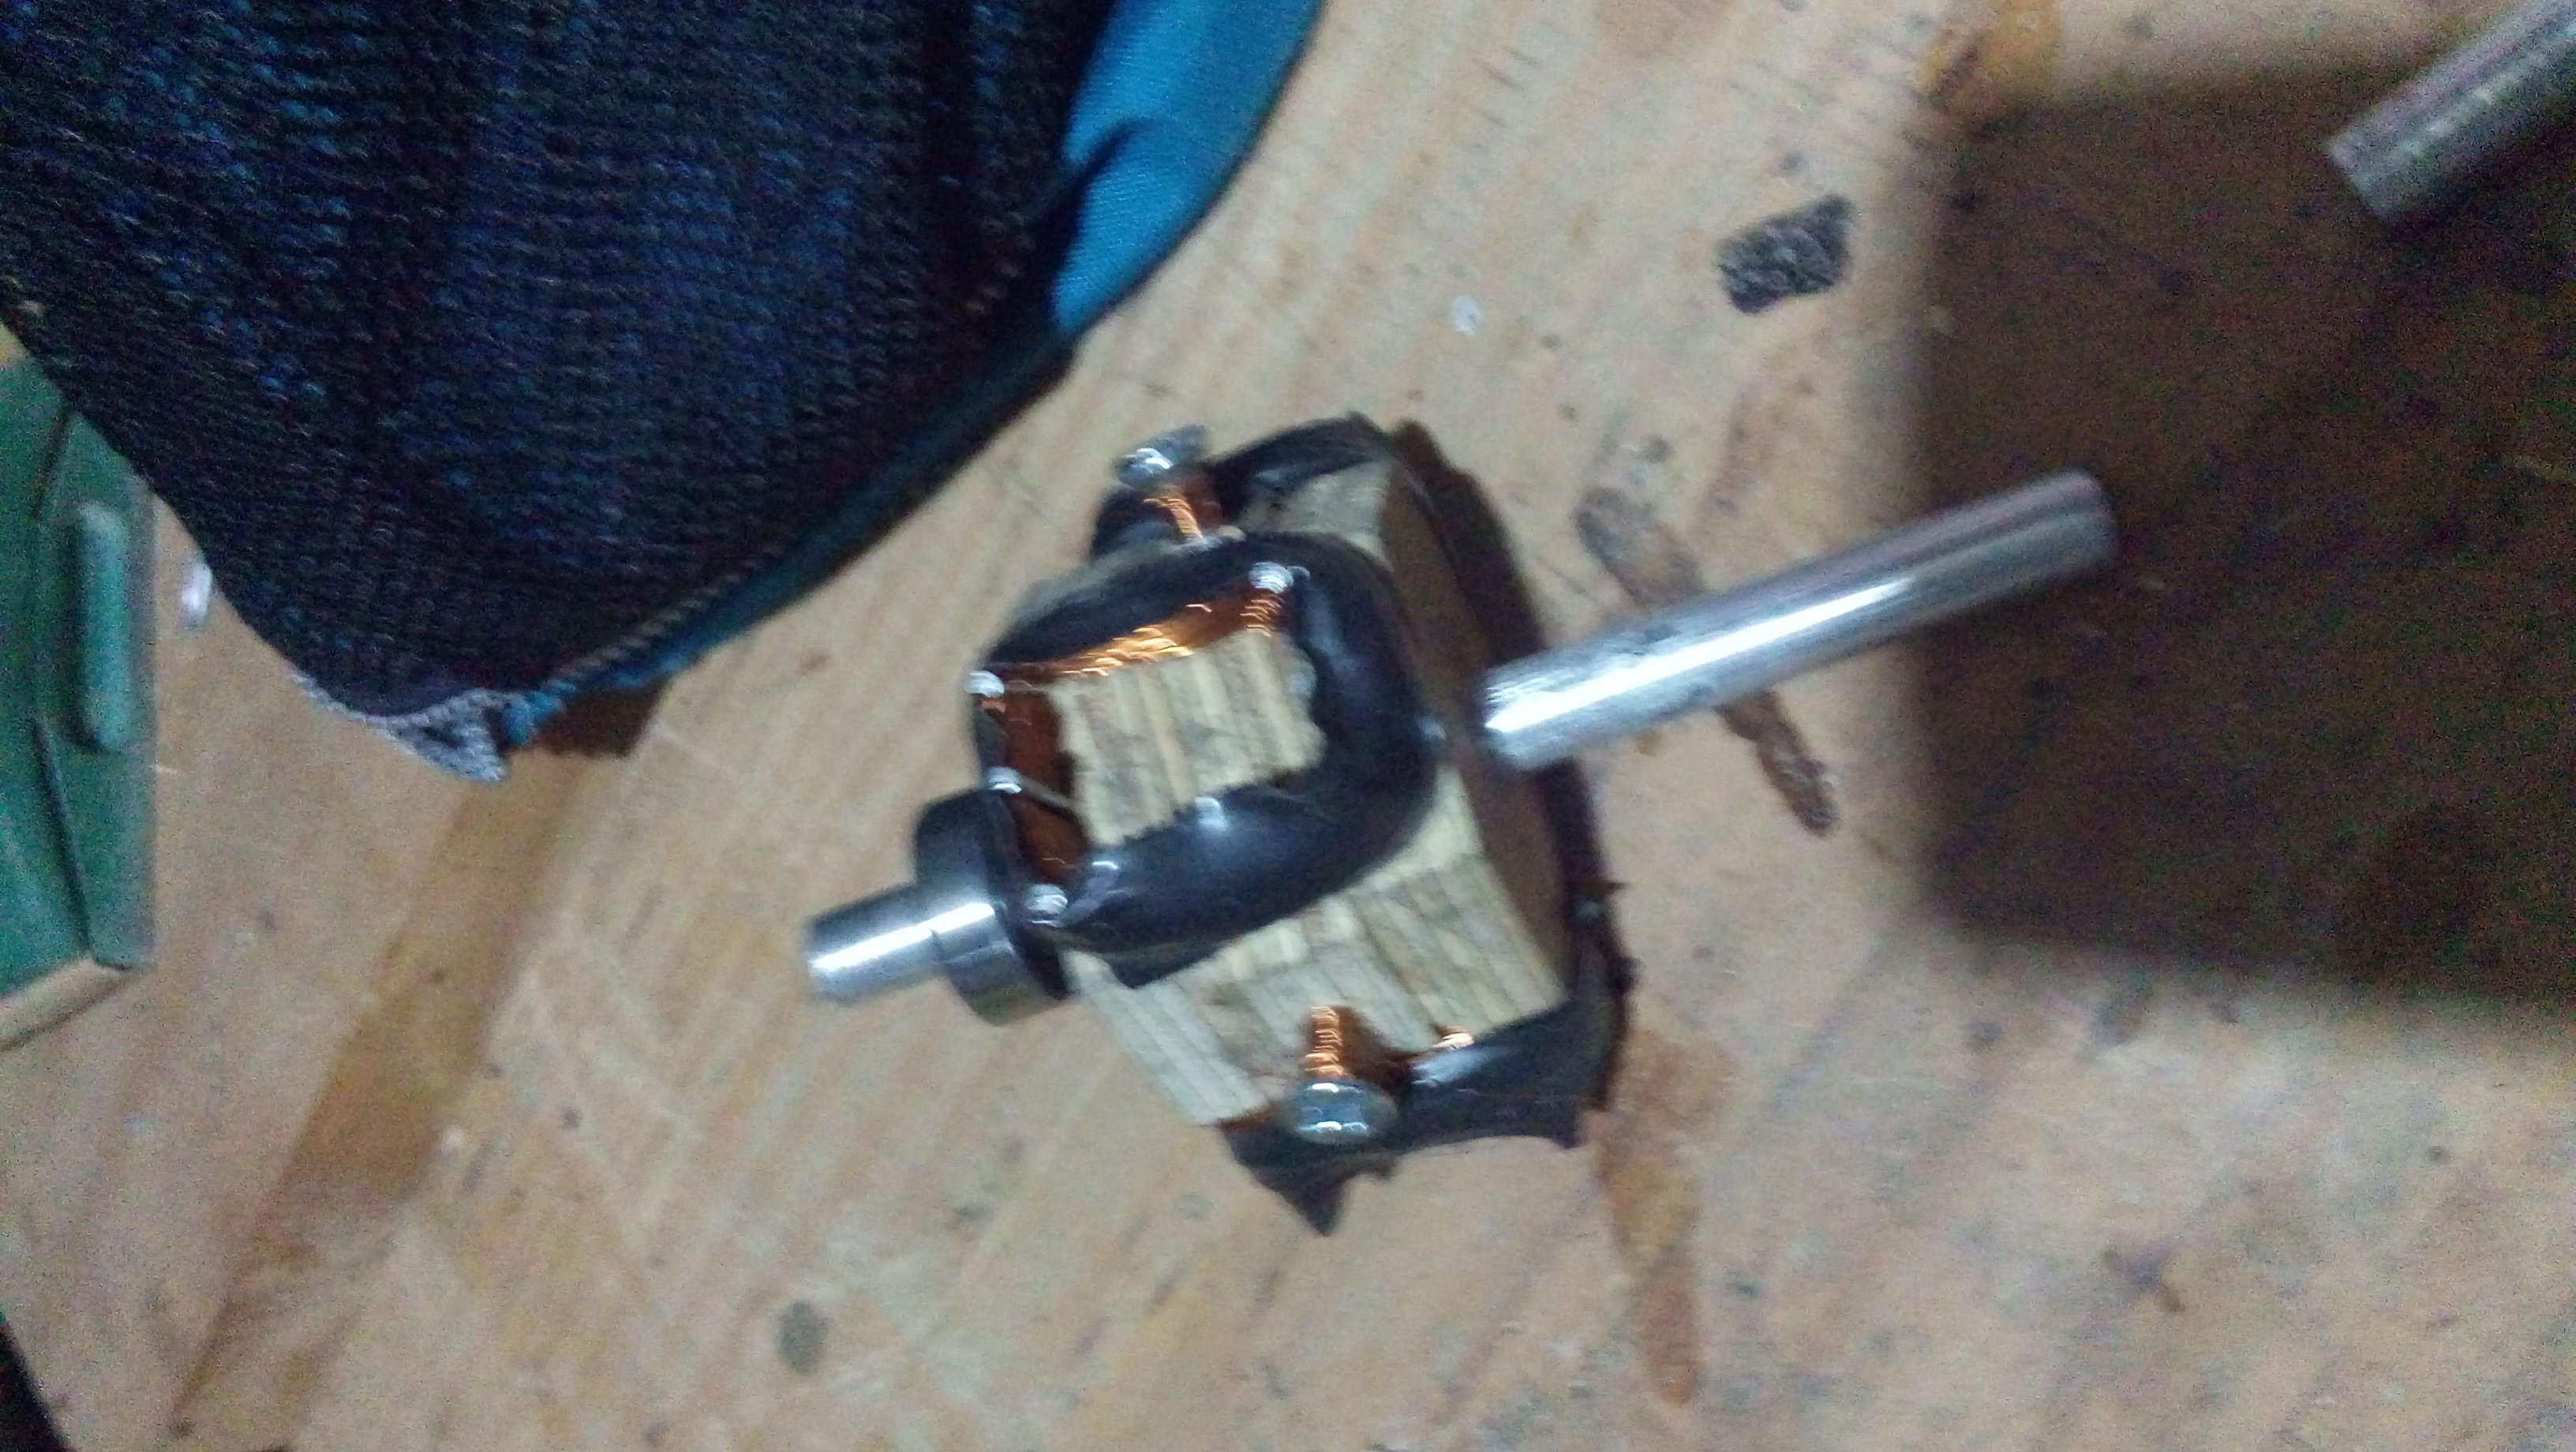
\includegraphics [scale=0.10]
{./img/20160228_190829.jpg}
\end{figure}

\begin{figure}[!htbp]
\caption{Ensamble del primer dise\~no}
\centering
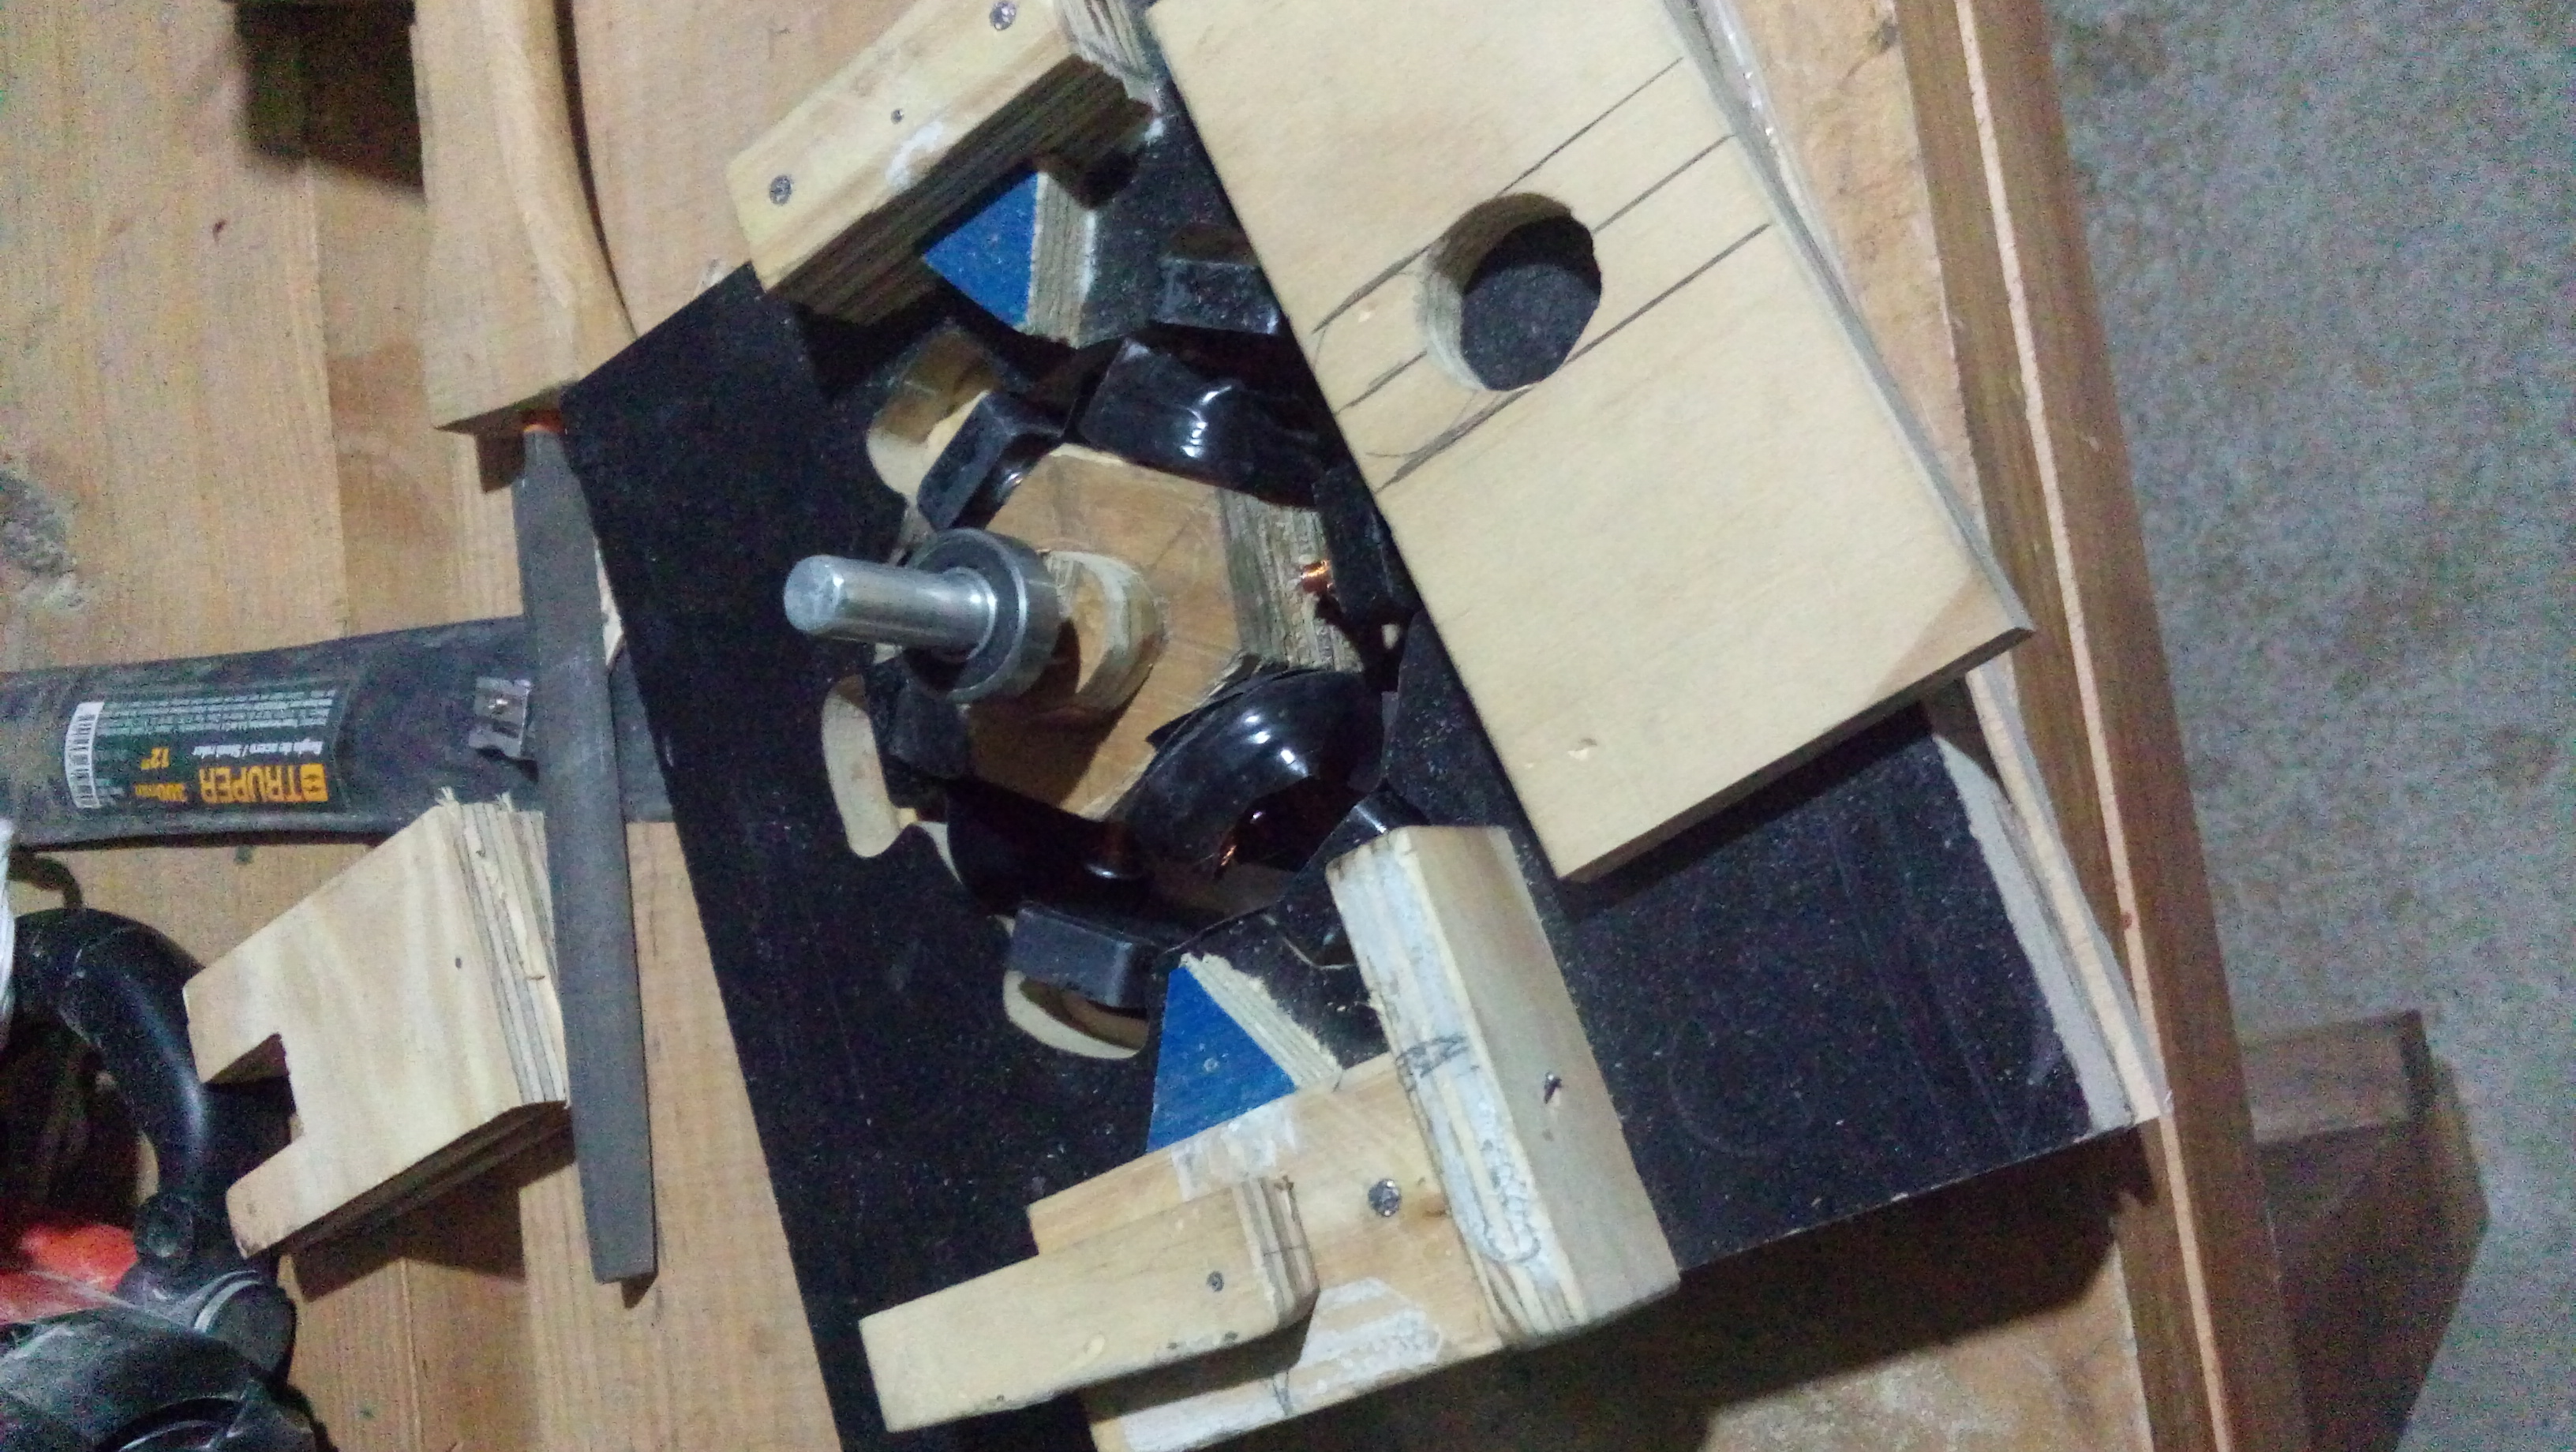
\includegraphics [scale=0.10]
{./img/20160228_204710.jpg}
\end{figure}

\begin{figure}[!htbp]
\caption{Segundo modelo}
\centering
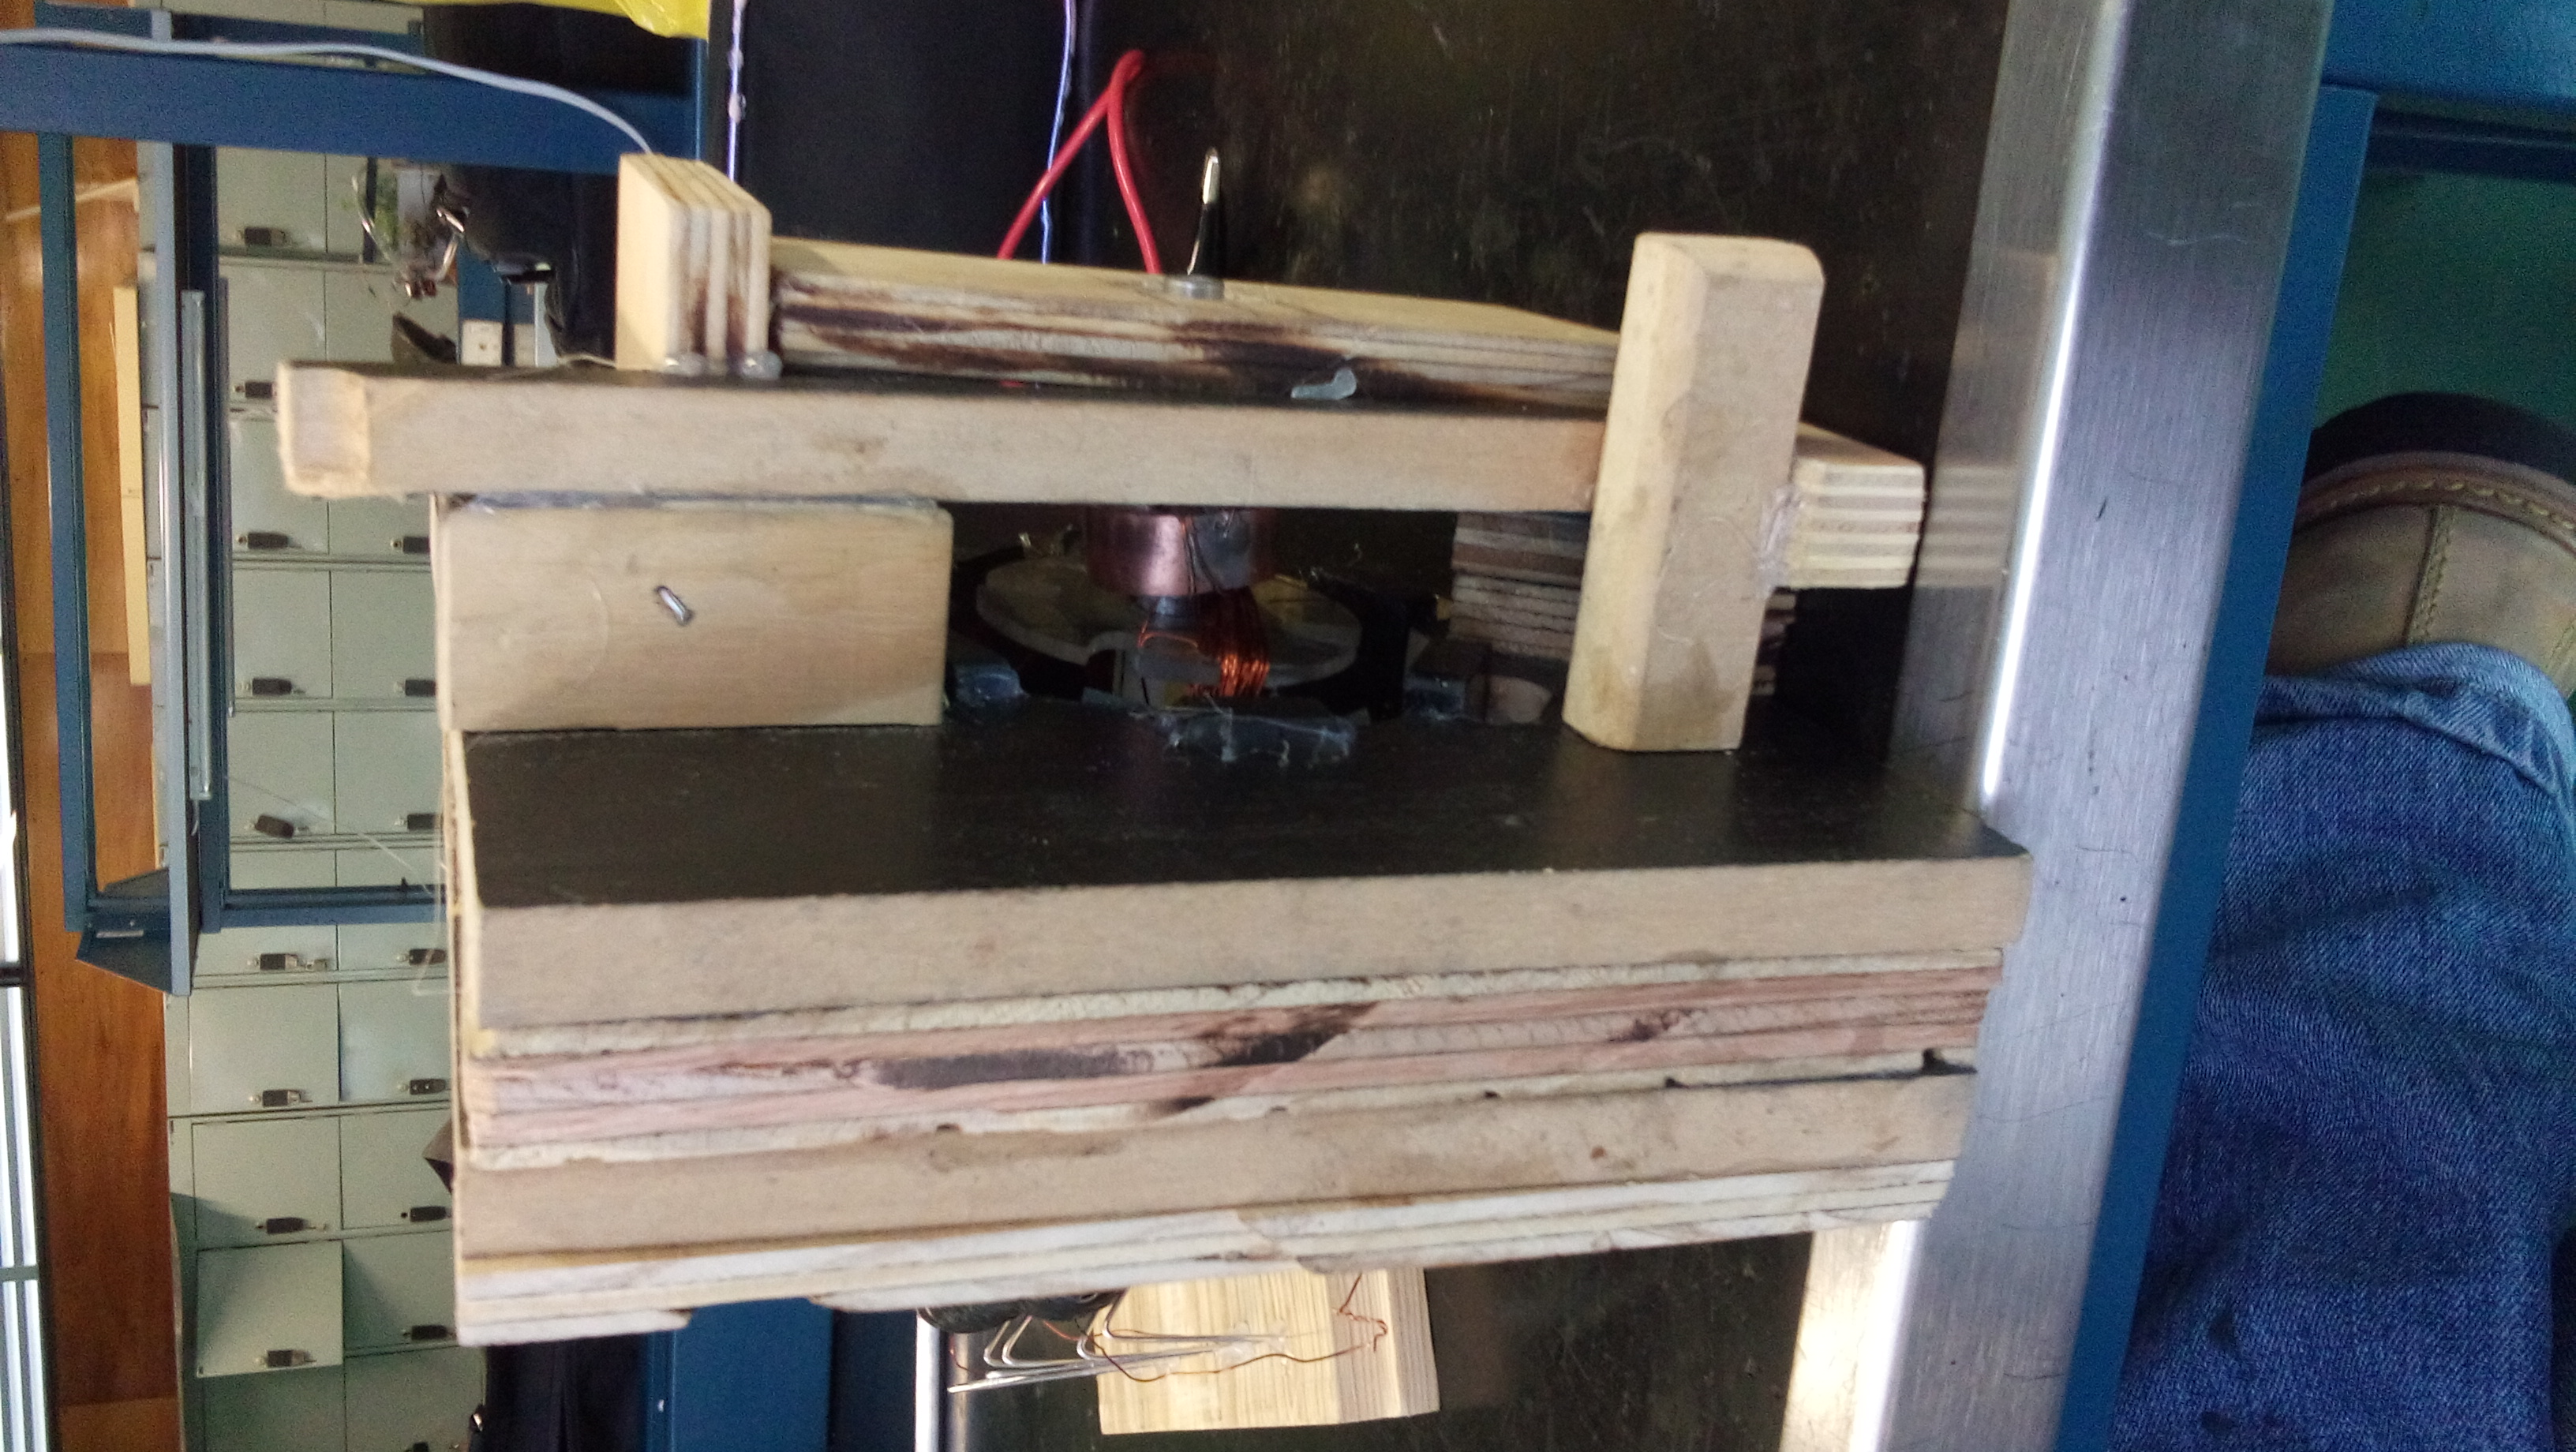
\includegraphics [scale=0.10]
{./img/20160301_134958.jpg}
\end{figure}

\begin{figure}[!htbp]
\caption{Bobinas}
\centering
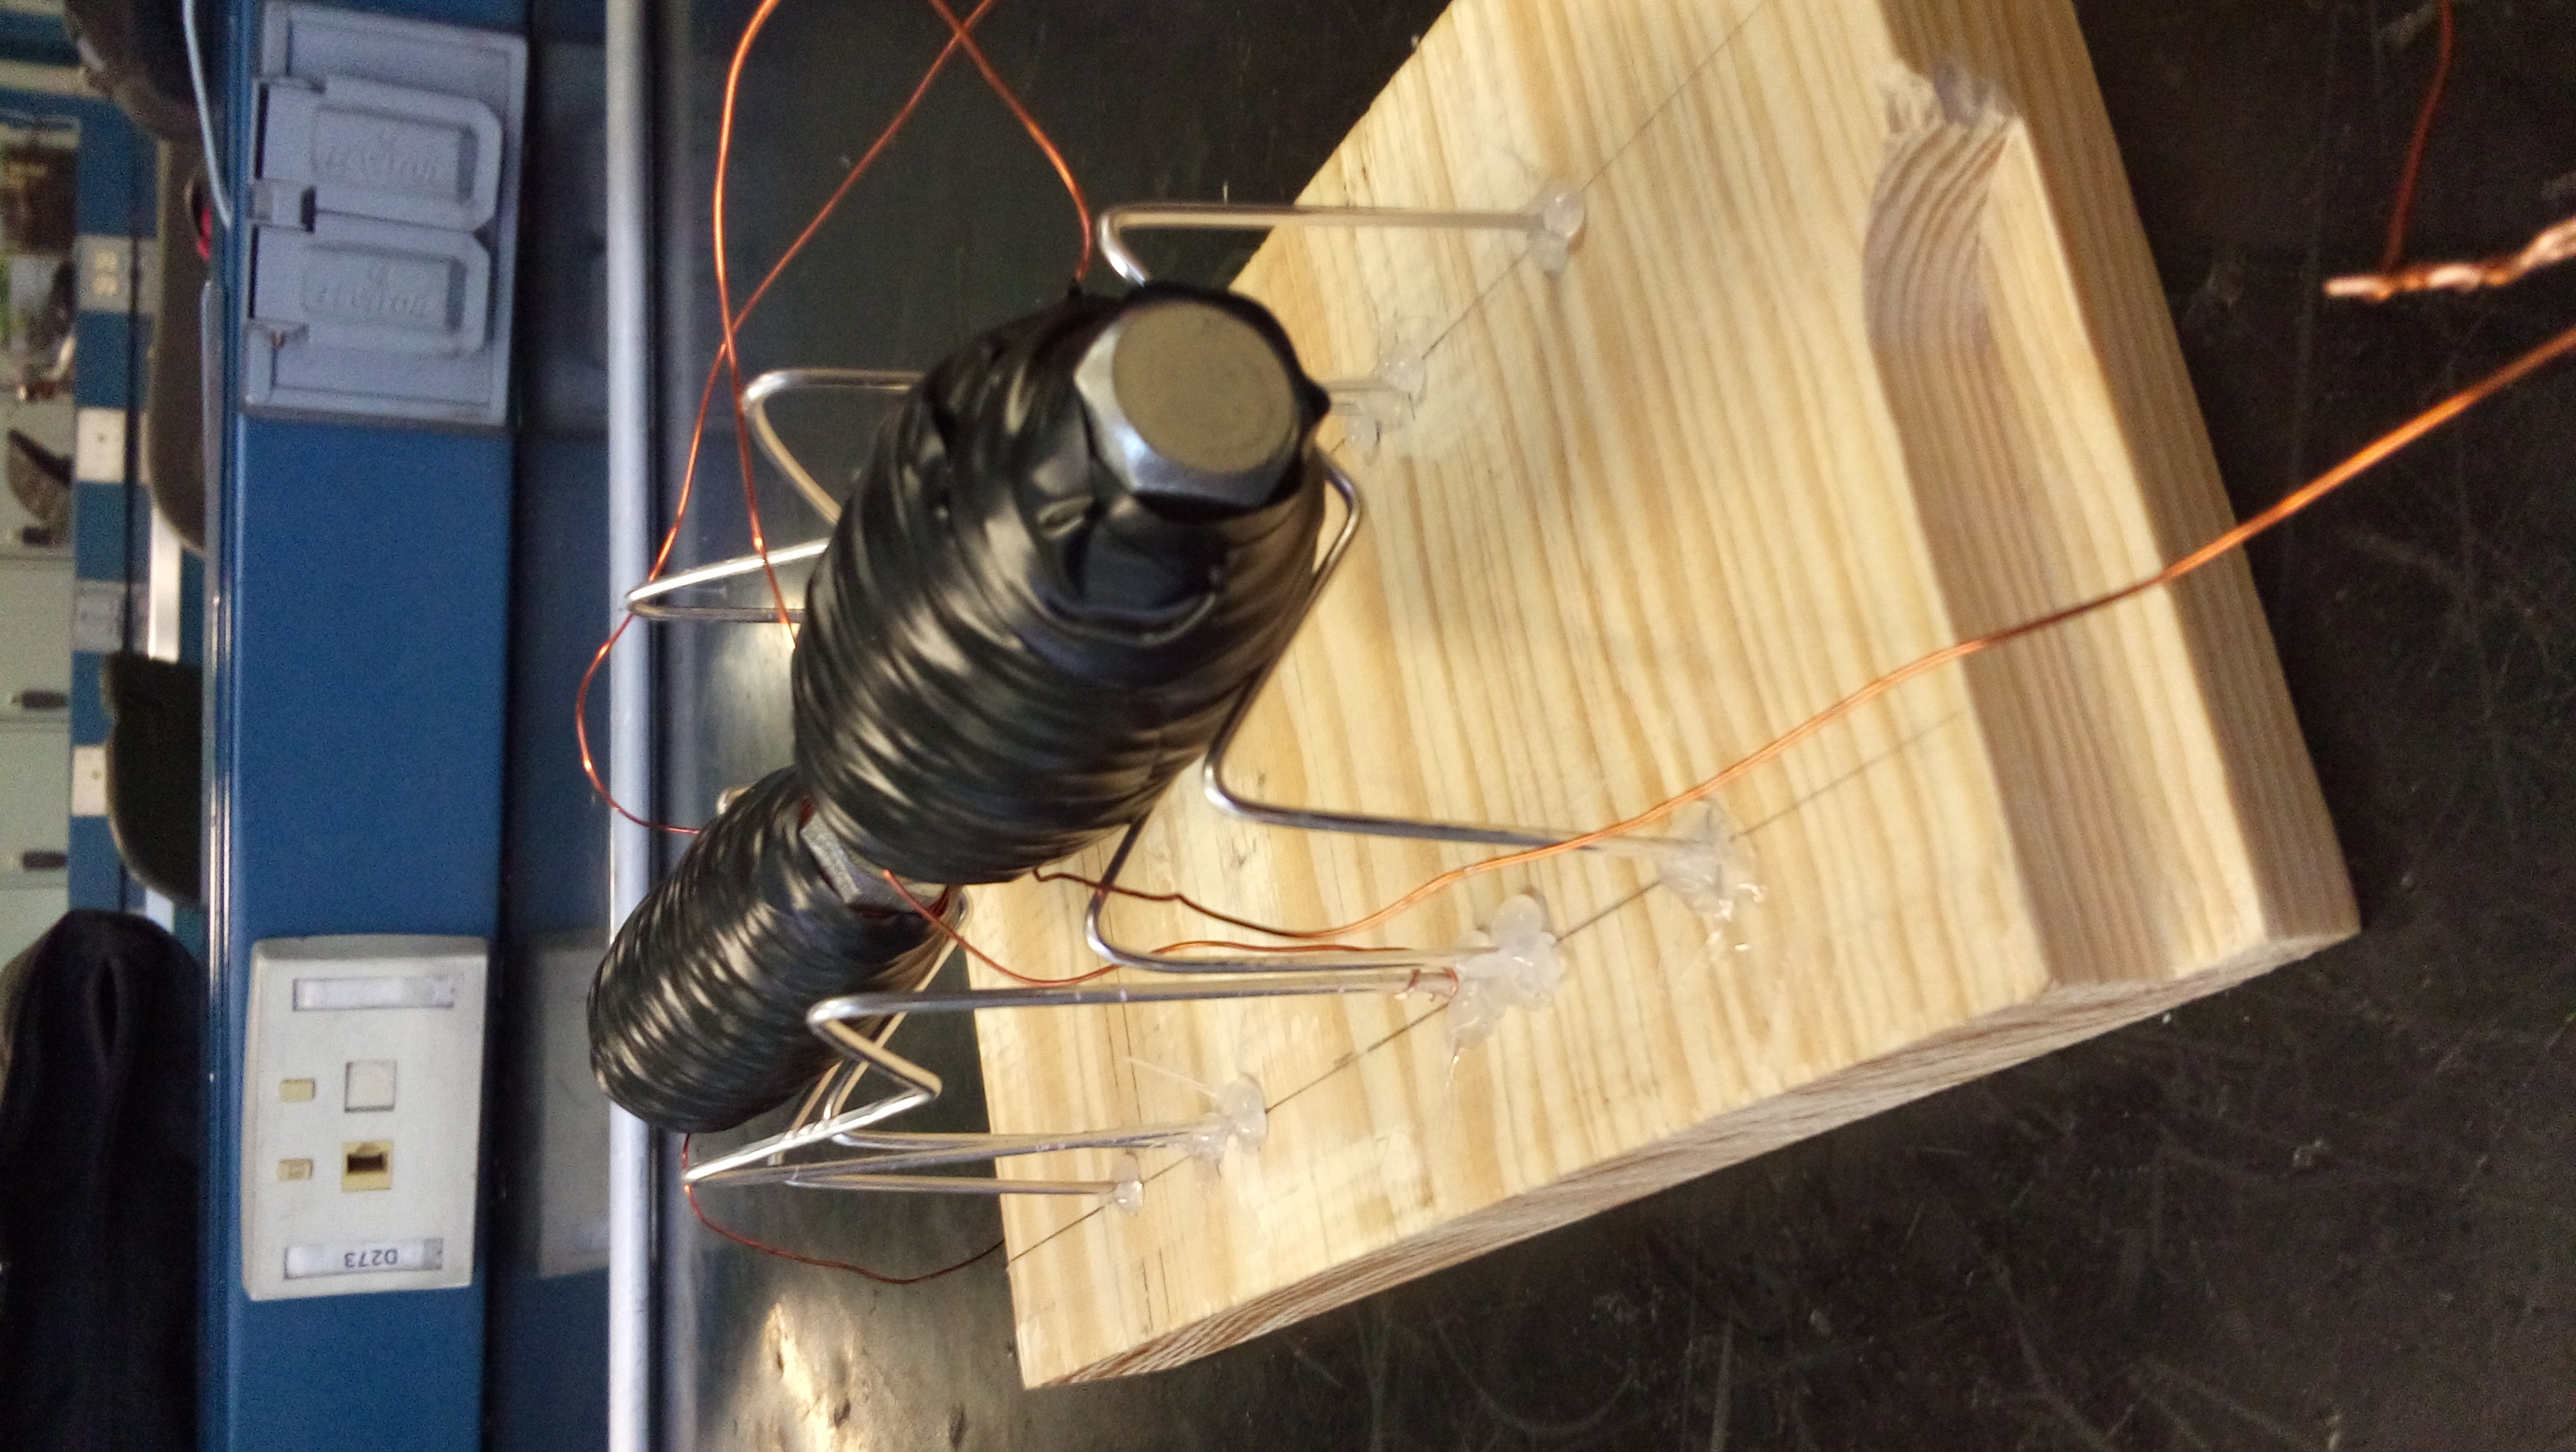
\includegraphics [scale=0.10]
{./img/20160301_135006.jpg}
\end{figure}

% \pagebreak